\clearpage % Ends the current page and causes all figures and tables to be printed

\begin{figure*}[p] % The * makes the figure span both columns, p places the figure on a float page
  \begin{center}
 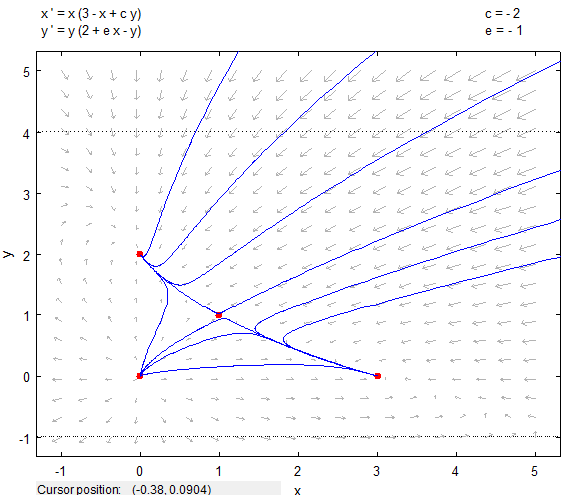
\includegraphics[width=0.6\textwidth]{images/ppcomp.png}
  \end{center}
  \caption{Phase portrait for the competitive system. This has an unstable focus at $(0,0)$, a saddle point at $(1,1)$ and two stable nodes at $(0,2)$ and $(3,0)$. \newline All phase portraits were generated using Matlab (\texttt{http://www.mathworks.com}) and pplane8 (\texttt{http://math.rice.edu/\textasciitilde dfield/}). Equilibriums are marked by red dots, and trajectories by solid blue lines.}
  \label{fig:ppcomp}
\end{figure*}

\begin{figure*}[p] % The * makes the figure span both columns, p places the figure on a float page
  \begin{center}
 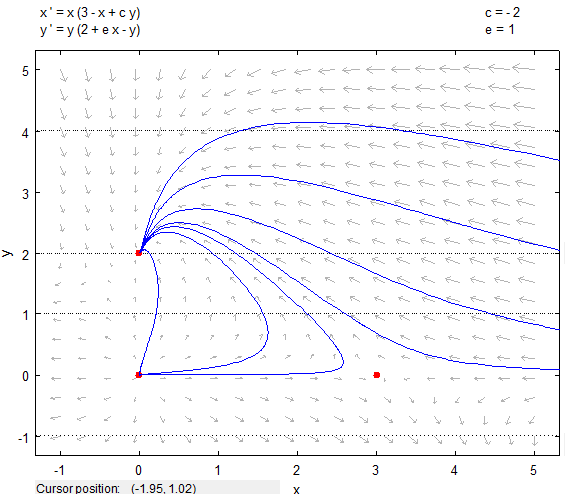
\includegraphics[width=0.6\textwidth]{images/ppy.png}
  \end{center}
  \caption{Phase portrait for the "$y$-predator" system. This has an unstable focus at $(0,0)$, a saddle point at $(3,0)$ and a stable node at $(0,2)$. The second saddle point at $(-\frac{1}{3},\frac{5}{3})$ is not considered since that point does not make physical sense (population must be $\geq 0$). }
  \label{fig:ppy}
\end{figure*}

\begin{figure*}[p] % The * makes the figure span both columns, p places the figure on a float page
  \begin{center}
 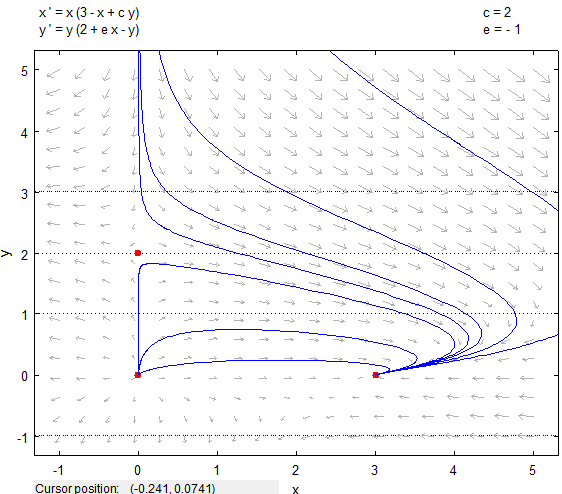
\includegraphics[width=0.6\textwidth]{images/ppx.png}
  \end{center}
  \caption{Phase portrait for the "$x$-predator" system. This has an unstable focus at $(0,0)$, a saddle point at $(0,2)$ and a stable node at $(3,0)$. The second saddle point at $(\frac{7}{3},-\frac{1}{3})$ is not considered since that point does not make physical sense (population must be $\geq 0$).}
  \label{fig:ppx}
\end{figure*}

\begin{figure*}[p] % The * makes the figure span both columns, p places the figure on a float page
  \begin{center}
 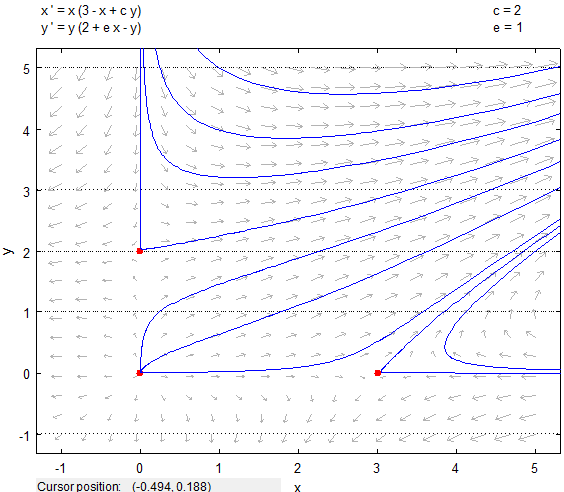
\includegraphics[width=0.6\textwidth]{images/ppsymb.png}
  \end{center}
  \caption{Phase portrait for the symbiotic system. This has an unstable focus at $(0,0)$ and two saddle points at $(0,2)$ and $(3,0)$. The third saddle point at $(-7,-5)$ is not considered since that point does not make physical sense (population must be $\geq 0$).}
  \label{fig:ppsymb}
\end{figure*}

\begin{figure*}[p] % The * makes the figure span both columns, p places the figure on a float page
  \begin{center}
 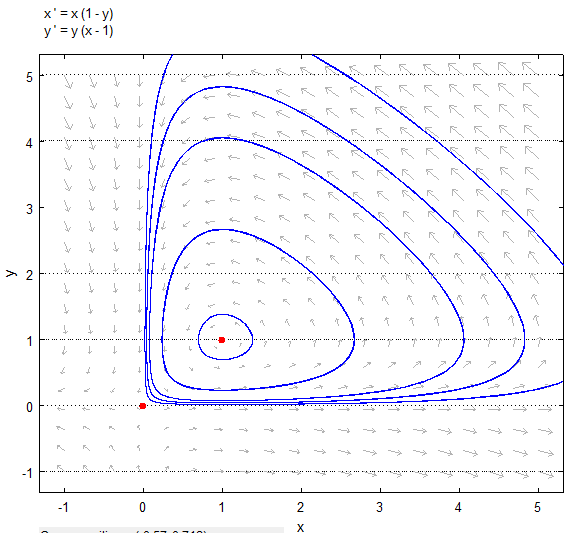
\includegraphics[width=0.6\textwidth]{images/ppcircle.png}
  \end{center}
  \caption{Phase portrait for the system in exercise 3. This has an saddle point at $(0,0)$ and a center point in $(1,1)$, as shown in section (4).}
  \label{fig:ppcircle}
\end{figure*}

\begin{figure*}[p] % The * makes the figure span both columns, p places the figure on a float page
  \begin{center}
 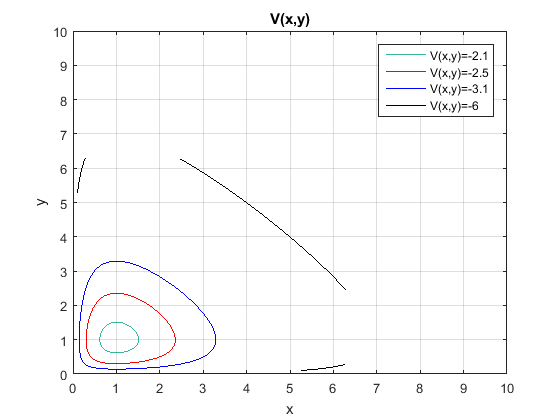
\includegraphics[width=0.75\textwidth]{images/Vlevelsets.png}
  \end{center}
  \caption{Level sets of $V(x,y)$, described in section (4). Notice that the level set $V(x,y)=-c$, for $c$ sufficiently big, is not a closed curve. For $c = -2.5$ we have a simple, closed, bounded curve. The curve $\gamma = \{(x,y) \in \mathbb{R}, \varepsilon> 0 : V(x,y)=-2-\varepsilon\}$ for $\varepsilon \to 0$ becomes a circumference centred in $(1,1)$. This behaviour can be seen for $V(x,y)=-2.1$, as shown in the figure.}
  \label{fig:vlevelsets}
\end{figure*}

%%%%%%%%%%%%%%%%%%%%%%%%%%%%%%%%%%%%%%%%%%%%%%%%%%%%%%%%%%%%%%%%%%%%%%%%%%%%%%%%%%%
% From example 1
%%%%%%%%%%%%%%%%%%%%%%%%%%%%%%%%%%%%%%%%%%%%%%%%%%%%%%%%%%%%%%%%%%%%%%%%%%%%%%%%%%%

% \begin{figure*}[p] % The * makes the figure span both columns, p places the figure on a float page
%   \begin{center}
%   \end{center}
%   \caption{Step response of the two systems. The figure should have a caption that briefly explains what it shows. The color, symbol and line type should be selected such that the lines can be distinguished when printed in black and white. The lines should be annotated either in the plot, in a legend, or in the caption. The axis should have a label in which the units are given. The figure should be sufficiently large, clear, easy to understand and only contain essential information.}
%   \label{fig:prestanda}
% \end{figure*}

% \begin{table*}[p] % The * makes the table span both columns, p places the table on a float page
% \caption{Jacobian matrix $A$ of the linear system $\dot{\textbf{x}} = A \textbf{x}$. The table should have a caption that briefly explains what it shows.}
% \label{tab:JacobianMatrix}
% \begin{center}
% \begin{tabular}{@{\vrule height 10.5pt depth4pt  width0pt}|c|c|c|c|}
%     \hline
%      $-2.46$ & $0$ & $-1.73$ & $0$ \\ \hline
%      $0$ & $-2.553$ & $0$ & $2.774$ \\ \hline
%      $0$ & $6.172$ & $-10$ & $7.333$ \\ \hline
%      $1.767$ & $-0.357$ & $5.714$ & $-6.074$ \\ \hline
% \end{tabular}
% \end{center}
% \end{table*}


% \begin{figure*}[p] % The * makes the figure span both columns, p places the figure on a float page
%   \begin{center}
%   \end{center}
%   \caption{Phase portrait of the system in \eqref{eqn:PPSystem}, which has a stable focus at \mbox{(0,0)} and a saddle point at \mbox{(-0.5,0)}. Both equilibriums are marked by large dots and selected trajectories are marked by solid lines. Trajectories starting within the shaded region end at the stable focus. This figure was generated in
%   Matlab (\texttt{http://www.mathworks.com}) using pplane7 (\texttt{http://math.rice.edu/\textasciitilde dfield/}).}
%   \label{fig:pplane}
% \end{figure*}